% !TEX root = ../main.tex

\chapter{Proof construction}
In this chapter, we will construct the proof of liabilities and the proof of inclusion. 
We will go through different circuit designs to find the optimal proof of inclusion and proof of liabilities.
We will start by describing a standard proof of liabilities and inclusion, which we will then optimize and propose novel solutions using recursion schemes.
We will propose a proof of inclusion derived from existing literature and a novel proof of liabilities. 


\section{Constants}
Before constructing the circuits, we need to define the constants that will be shared between the
different circuits.


\subsection{Circom} 

Circom is a domain-specific language designed to create arithmetic circuits specifically utilized in zk-SNARKs. These proofs verify calculations without revealing private data, like proving we have funds without showing our account.
Within Circom, circuit code is written to define the desired constraints. One notable distinction from other languages is the utilization of signals and templates.
Templates can be conceptualized as functions that operate as circuits. The primary template receives signals as inputs and produces other signals as outputs. Signals can be classified as either public or private.
Assigning a value to a signal contributes to the constraint system and the witness calculation process.
Input and outputs are signals, and we can have additional intermediate signals.
In Figure 4.1, the template can be used to calculate the square of an input. The template creates a constraint $in * in = out$.

\begin{figure}[h]
   \centering
   \begin{lstlisting}[language=C, basicstyle=\ttfamily\small]
 template Square() {
 signal input in;
 signal output out;
 out <== in * in;
 }
   \end{lstlisting}
   \caption{Template and Signal Example}
   \label{fig:square}
   \end{figure}

 During circuit compilation, constraints are generated in r1cs format. Additionally, compiling a circuit produces a witness file containing the data essential for verifying the constraints and demonstrating the circuit's correct behavior.


\subsection{MiMCSponge} 
MiMCSonge is a standard hashing algorithm often used in zero-knowledge protocols. It was chosen because it is secure and well-integrated with Circom.
The hash function is $F_i(x) = (x + k + c_i)^3$, where $i$ is the number of rounds, $k$ is a fixed constant, and $c_i$ is a constant specific for a round.
In our implementation, we use $i = 220$ and $k = 1$, both standard values. We use four inputs: the two sums and two hashes of the children. 
The hash function is a sponge construction. This is a modern way to do hash functions where it is easier to do security assertions. 
It does the 220 rounds on the first input, then adds the second input and starts over again.



\subsection{Constraints} 


A zero-knowledge circuit generally enforces two types of constraints: range checks and arithmetic constraints. 
The simplest arithmetic case is when we define a value in Circom, such as $a = b + c \bmod q$, where $q$ is a parameter of the elliptic curve Circom uses. 
Circom compiles the assignment to create an arithmetic constraint that verifies the equality holds within the finite field $q$.

A range check verifies that a value lies within specified bounds. This is necessary because operations occur in a finite field. This means an overflow would cause the value to return to 0.
We limit the range of the values to prevent overflow. This is critical because an overflow would change the balance sum we are trying to prove.
Range checks are critical, especially for multiplications, as the product of two numbers can grow exponentially, leading to overflows much faster than additions.
We limit the range of values to ensure no overflow occurs, preserving the correctness of computations.

In Circom, the range check constraint is transformed into an arithmetic constraint. 
For instance, to verify $x < n$, we can use a library function like \texttt{lessThan}. 
This function decomposes the numbers into their binary representations and performs a series of bit equality checks to determine the result. 
Circom compiles these bit equalities into arithmetic constraints. 
A more straightforward way to prove a small number is to prove that the leading bits are 0. Proving that an $n$-bit number has $i$ leading zeros demonstrates it is less than $2^{n-i}$. 
We can do the sum of the leading bits and prove it equals 0.
For instance, if we add $n$ balances where each balance is $k$ bits, then the sum can never exceed $n \cdot (2^k - 1)$

As mentioned before, in Circom, we use a specific variable type called a signal. When we assign a value to a signal, a constraint is usually created.
There is a way to assign value without creating a constraint, but it adds complexity, and we have never used it in this paper. 
Therefore, it is safe to assume that assigning a value to a signal creates a constraint. 
Every variable in this chapter will be of the type signal.
This means that the values will be constrained automatically as we define them. 
\subsection{SnarkJS} 

SnarkJS is a JavaScript library that provides tools for working with zk-SNARKs, including compiling circuits defined in Circom. 
After writing our circuit using Circom, SnarkJS generates the r1cs and witness file for it. It then uses those files to create the zk-SNARK proof.
SnarkJS also provides utilities for verifying the proofs.

\subsection{Benchmark} 
We use Groth16 as a SNARK design choice because it is simple and fast. 
We will benchmark the circuits using the prover time and verifier time. The prover time does not include the time to generate the setup.
The setup needs to be generated for every circuit, but it only needs to be generated once. This is why we exclude it from our benchmarks.
The prover time is the time it takes to generate the proof, including generating and folding the constraints when we use the folding scheme. 
The verifier time is the time to verify the proof.

As mentioned in the \hyperref[subsec:plc]{KZG} section, a trusted setup must precompute values. These values need to remain a secret or, even better, destroyed.
This introduces a potential vulnerability, as you need to think about who will do the setup. Typically, multi-party computation ceremonies are used.
In practice, someone could use a universal setup like PLONK, which makes key generation easier because we only need one for every circuit. Groth 16 requires one secret per circuit.
Someone could also use a transparent setup (STARKS), which does not require any secret.

\subsection{Tree construction}
The proof is based on constructing a Merkle tree, where the leaves are the users' balances and hashes. The tree's root is the root hash and root sum, where the root sum is the sum of all balances or total liabilities.

The size of the tree is dynamic with the number of users. For instance, if we have $2^5 - 10$ users, we will use a tree of 5 levels. This means we will
have 10 empty nodes. We will use an empty hash and zero as the empty nodes' values. Those values are valid inputs for the MiMCSponge hash construction
and will give a valid hash as an output. An empty node has no impact on the state of the tree.

The size of the tree decides the number of constraints. We need a separate setup for every tree size, but those setups are precomputed. 
For instance, a power of Tau of 8 (8 refers to the number of degrees of the QAP polynomial) can handle up to 256 constraints, 9 for 512 constraints, and so on.


\section{Proof of liabilities}
\label{subsec:pl}
The proof of liabilities operates on a list of balances and a list of email hashes as private inputs kept private to preserve privacy. 
The proof of liabilities aims to generate a Merkle root without revealing additional information about the users and their balances.
The first purpose of the circuit is to validate that all values are non-negative and that all balances fall within a specified range.
Since operations occur within a finite field, these verifications are crucial to prevent overflow or underflow issues.
An insolvent exchange can deceive a proof of solvency by exploiting overflows in finite field arithmetic. 
It can encode negative balances as large positive values that will reduce the size of the liabilities. 
For instance, assume the total liabilities of an exchange is $1000$. It can encode a negative value $-400$ as a large positive value $q - 400$. 
The exchange would then add this false balance to the tree, and the new total liabilities would be $600$. 
The range-check constraint prevents this type of attack. A balance is assured to contribute positively to the sum, or at least not negatively (if the balance is 0). 
Therefore, there is no incentive to encode false balances for the exchange.

Subsequently, the proof of liabilities constructs a Merkle tree and outputs the total balance sum and the root hash of the Merkle tree.
The pseudocode for the circuit is found in Appendix~\ref{subsec:plc}.


\paragraph{Inputs}
\begin{itemize}
   \item List of balance (private): List of user balances, kept secret to protect individual amounts.
   \item List of email hash (private): User emails, hidden to protect identities and used in the Merkle tree. It is included to prevent \hyperref[subsec:ca]{clash attacks}.
   \end{itemize}


\paragraph{Outputs}
\begin{itemize}
   \item Balance Sum: Total of all balances, showing overall liabilities without revealing individual amounts.
   \item Root hash: Merkle tree's top value, used to check the tree's integrity.
   \item All small range: True if balances are within a safe range.
   \end{itemize}


This proof of liabilities operates as intended because it returns the sum of the liabilities and the root hash, ensuring we cannot alter any values inside the Merkle tree. 
The Merkle tree is hidden, so we do not give any information about users and their balances.
The root hash will be used to verify the inclusion of the balances.

The balance sum would be a private output in a complete proof of reserves. We would have another circuit proving that the sum of liabilities is smaller
than the sum of assets without revealing the balance.

The circuit follows the zero-knowledge \hyperref[subsec:zkp]{properties} we highlighted previously. 
\paragraph{Properties}
\begin{itemize}
   \item Completeness: A Merkle sum tree will be produced alongside the proof if the input balances are non-negative and within the range. The arithmetic constraints and range checks enforce this.
   \item Soundness: A valid proof cannot be produced if any input balance is negative or outside the range. Moreover, the Merkle sum tree cannot produce an inaccurate root hash and sum if the inputs are valid due to constraints ensuring sum accuracy and Merkle path integrity.
   \item Zero-Knowledge: The verifier learns only the public outputs and does not gain any information about the individual inputs. The hash provides not useful information.
   \end{itemize}


\section{Proof of inclusion}
\label{subsec:pi}
The proof of inclusion aims to prove that a user's balance is included in the Merkle tree created in the proof of liabilities.
To do so, the exchange reveals the leaf associated with the user, which is the hash of the user's email and balance.
This data will be the public input to the circuit alongside the root data.
The exchange uses private inputs to show that the leaf is part of the tree. 
The circuit combines the user's data with the neighbors' data to show that the hash of the user's leaf is part of the hash of the Merkle root, showing at the same time that the user's balance is included in the total liabilities.
The neighbors' data refers to the data of the sibling nodes along the unique path from the user's leaf to the root.
It includes their sum, hash, and binary. The neighbors' binary variable indicates whether the neighbor is on the left or the right, which is needed to calculate the proper hashing order. 

In short, we use the generated hash root in the proof of liabilities to prove that the balance is included in the Merkle tree.
It checks if a path through the tree leads to the correct top value, proving the balance is included without revealing other data.
To prove that a user balance is included, it is sufficient to show that you know the Merkle path of that balance. 

If the exchange wanted to prove a leaf not included in the Merkle tree, it would not be able to do so. 

For the following figure, the blue nodes represent the value of the Merkle path.
We would have $neighborsSum=[29,61]$, $neigborsHash=[Hash(User1),Hash(L2,R2)]$ and $neighborsBinary=[0,1]$.
   \begin{figure}[H]
   \centering
   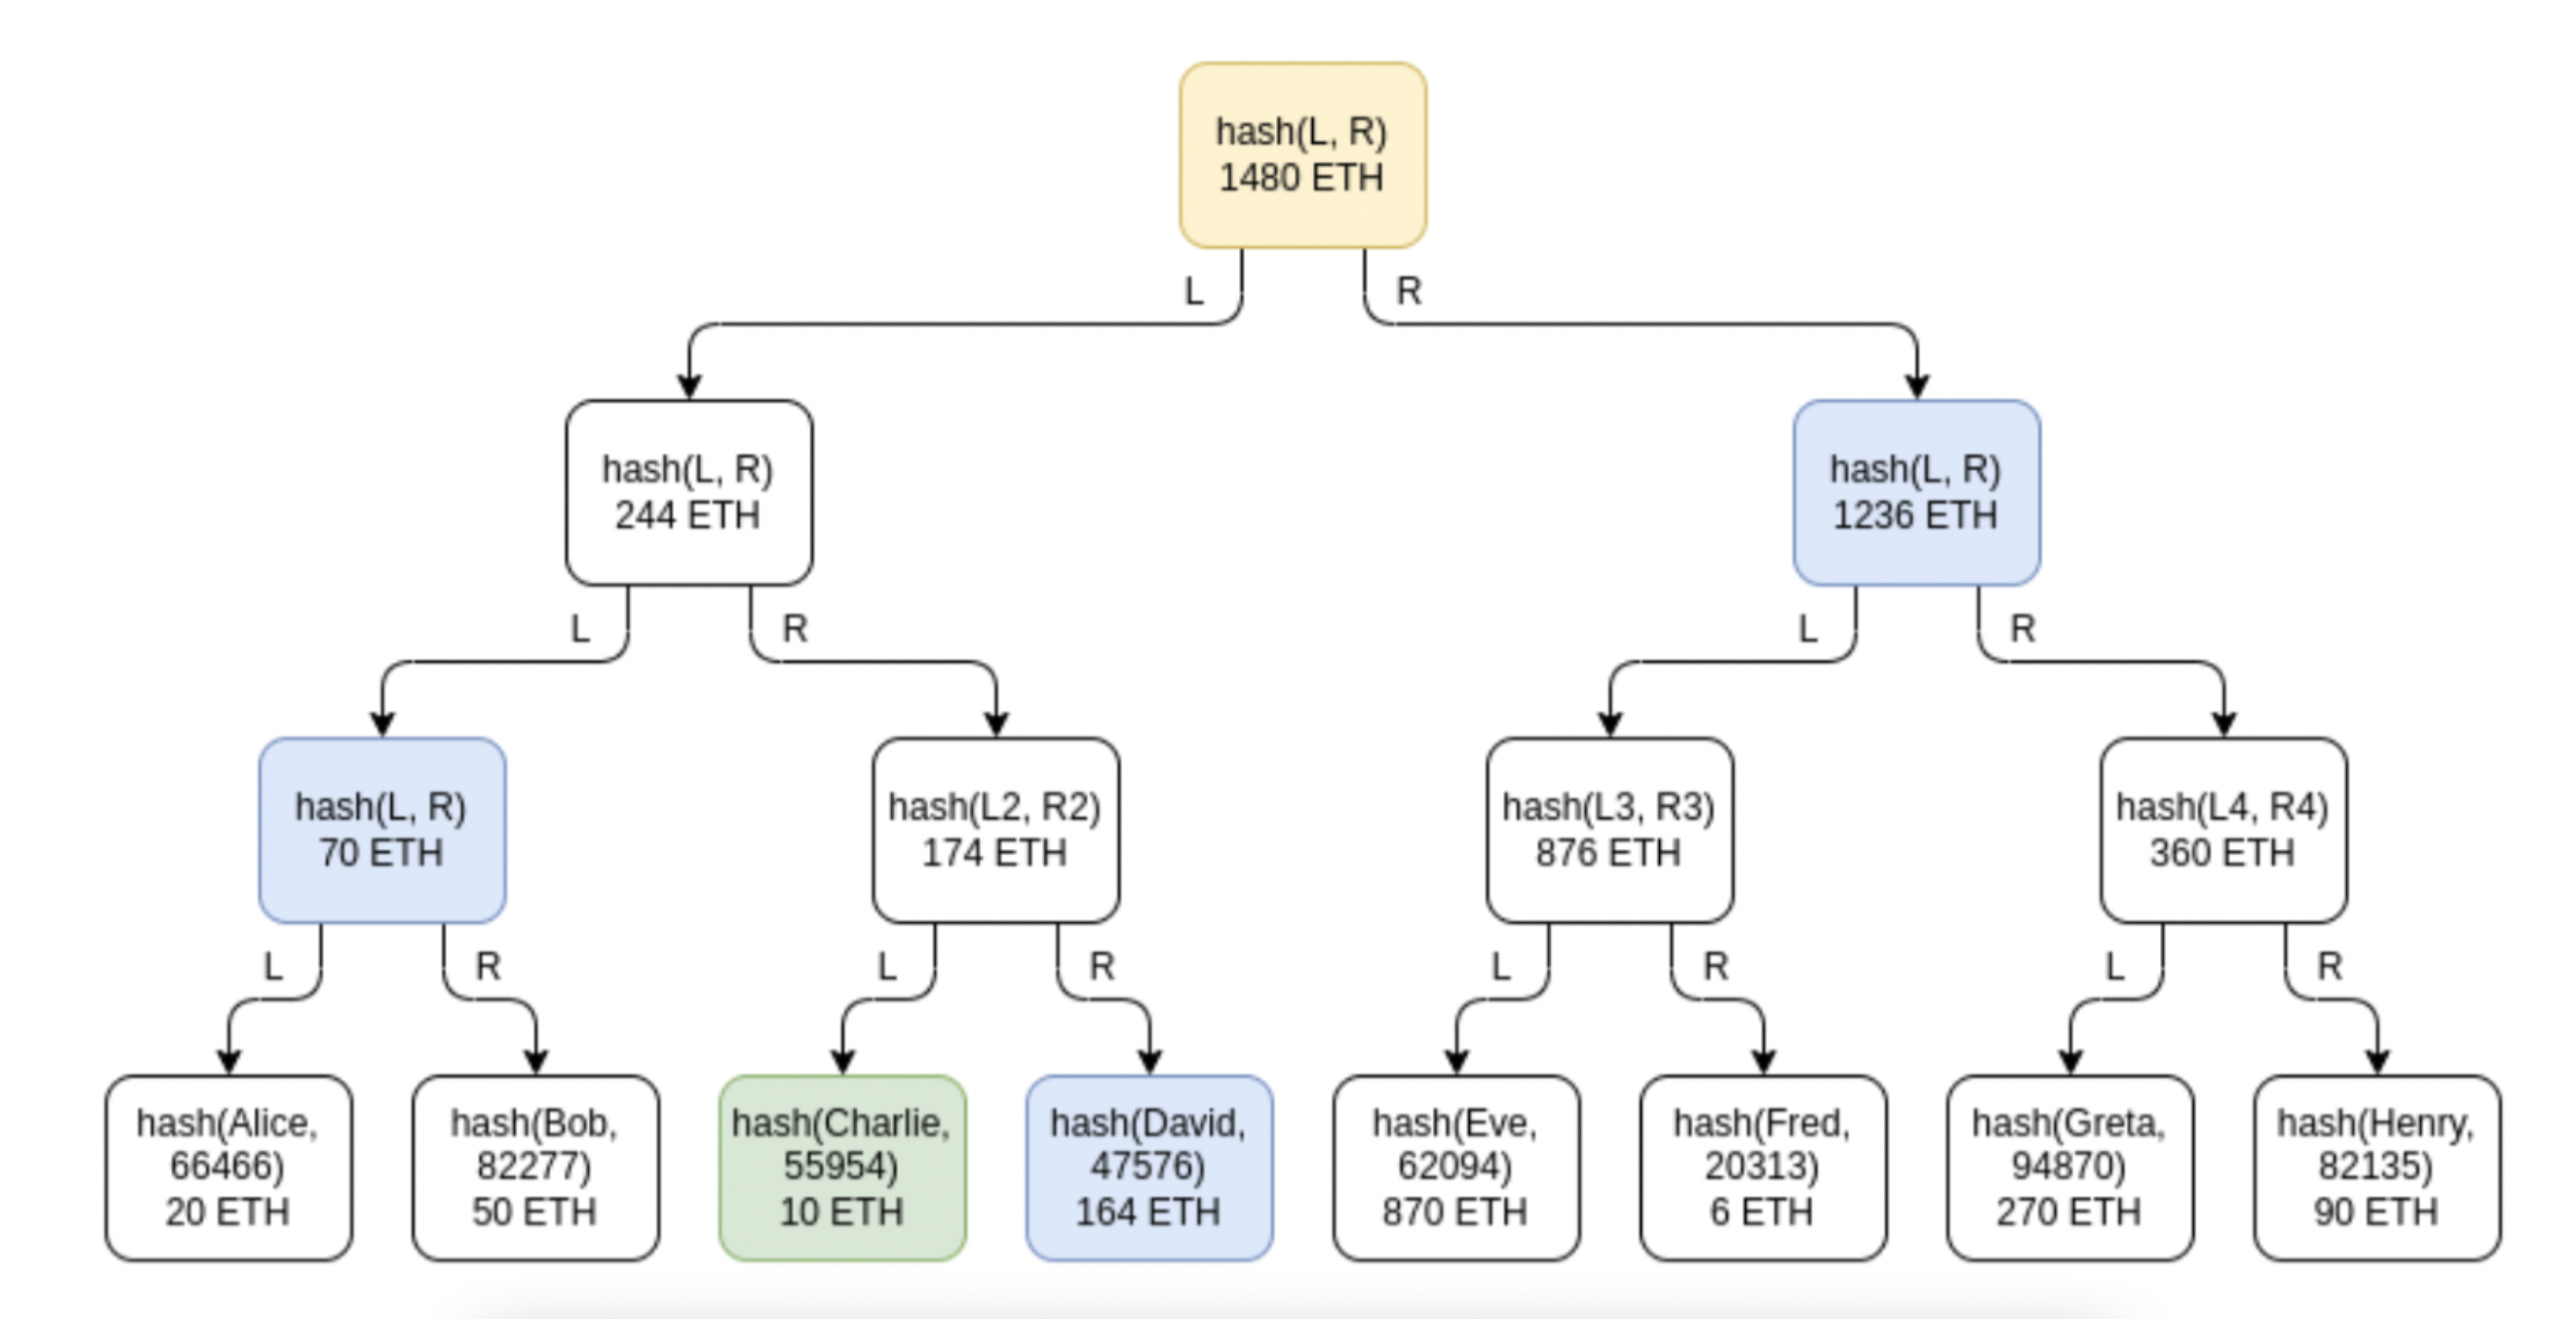
\includegraphics[width=130mm]{MerklePath.png}
   \caption{Merkle Path}
   \label{overflow}
   \end{figure}

\paragraph{Inputs}
\begin{itemize}
   \item List of neighbors sum (private): Sums of nearby tree nodes, kept secret to hide the tree's structure.
   \item List of neighbors hash (private): The hash value of nearby nodes, hidden for privacy.
   \item List of neighbors binary (private): Value showing if a neighbor is left (0) or right (1).
   \item Root hash (public): Merkle tree's top value, shared to identify the tree.
   \item Root sum (public): Total balance sum, shared for verification.
   \item User balance (public): User's balance, shared to prove it is included.
   \item User email hash (public): User email hash shared to identify the user.
   \end{itemize}

\paragraph{Outputs}
\begin{itemize}
   \item balanceIncluded: True if the balance is in the Merkle tree, confirming it is part of the data.
   \end{itemize}


The constraints in the circuit ensure that the path from the leaves to the root is correct. 
In the \hyperref[subsec:pic]{circuit}, we verify that combining the user balance, sum, and Merkle path gives the correct root hash and root sum. 
The circuit iterates over the path, combining values to recompute the root without revealing private data. 
No additional verifications are required since they have already been done for this root hash in the proof of liabilities. 
Constraints enforce the hash and sum calculations and path directions. 
Each new value in Circom is defined in a way that adds a constraint. For instance, the Root sum is constrained to be equal to its two children; the children are constrained to be equal to their two children, and so on.

Once again, the circuit follows the zero-knowledge \hyperref[subsec:zkp]{properties}. 

\paragraph{Properties}
\begin{itemize}
   \item Completeness: An honest prover can provide a valid Merkle path if a user's balance and email hash are included in the Merkle tree. This is verified by recomputing the public root hash and sum with constraints.
   \item Soundness: If the user's balance or email hash is not in the Merkle tree, or if the Merkle path is incorrect, no dishonest prover can produce a valid proof. This is because the hash function is collision-resistant.
   \item Zero-Knowledge: The verifier only learns whether the user's balance is included in the Merkle tree and nothing about the private inputs. All of the tree's internal structure is preserved with the SNARK privacy properties.
   \end{itemize}

\section{Vulnerabilities}
In this section, we discuss the potential vulnerabilities of our proofs.

\subsection{Clash attack}
\label{subsec:ca}
A clash attack can happen when two users have the same balance on the exchange, and the node of the tree is not linked to the user. 
For instance, if Alice and Bob both have 5.5 BTC on the exchange, the exchange could tell them that their balance is in leaf 157. 
It would then create a single proof of inclusion for leaf 157 and show it to Alice and Bob. Both would be happy because they would know that their balance is included in the total liabilities.

However, if we change leaf 157 for leaf x, where x is the hash of Alice's email, then the exchange cannot use the same leaf for Bob.

\subsection{Collusion}
Collaboration attacks occur when two exchanges collude to exchange funds to show that they are more solvent than they actually are.
This attack affects the proof of assets, indirectly affecting the proof of liabilities. Since we do not want exchanges to move funds around in between proofs,
we need to generate the proof of assets at a higher frequency and, therefore, the proof of liabilities at a higher frequency.

\subsection{User verification}
For the proof of liabilities to be valid, we must verify that the user's balance is included in the Merkle tree. 
The users must verify their proof of inclusion to validate the proof of liabilities. 
However, how many user verifications do we need to trust the proof of liabilities?

In this chart, we can observe the failure probability, which represents the likelihood that a dishonest prover gets away with misbehaving.
\begin{figure}[H]
   \centering
   \includegraphics[width=130mm]{FailureProbability.png}
   \caption{Failure Probability \cite{GP21}}
   \label{FB}
   \end{figure}
If we take the orange line, for example, where an exchange has 1 million users, the failure probability approaches 0 when over $4\%$ of users perform their verifications.
This might not seem like a reasonable threshold. However, this is only for one proof. We would need $4\%$ of users to verify every single proof. 
If we do a daily proof to avoid collusion, we are unlikely to reach the threshold every single day.

The last two attacks are the main vulnerability of the proof of inclusion and liabilities. 
To prevent these attacks, we need to generate the proof of liabilities more frequently and make it easier for the user to verify its proof of inclusion.

\section{Daily proof of liabilities}
In order to generate a daily proof of liabilities, we need to reduce the computational effort.
We aim to enhance our current \hyperref[subsec:pl]{circuit} by minimizing the work needed in subsequent rounds.
The first thing to explore is recursion proofs, specifically created to reduce the total computational effort across rounds.

\subsection{Recursion scheme}
The main advantage of the recursion scheme is that it streamlines the verification process. For instance, in the second round, we can prove the integrity of the current and all previous rounds.
However, this benefit comes with trade-offs. The first drawback is the increase in proof size, as it necessitates proving the current circuit and verifying the previous ones.

When considering the frequency of verification, having a fixed number of nodes verify the proof daily would be illogical, as it would be illogical to have the nodes verify the previous rounds every single day.
On the other hand, if the verification is not consistent or new nodes need to be able to quickly verify every proof, then aggregation becomes more appealing.

In our case, the priority is to produce daily succinct proofs. We need to ensure the integrity of every round while keeping the proof size to a minimum.
Therefore, having our nodes verify the circuit at every round without the computational overhead of the aggregated proof is sufficient.

\subsection{Other recursion proofs}
The recursion scheme is the only recursion proof that is proper in specific scenarios.
The other types of recursion proofs, namely Aggregation, Accumulation and Folding schemes, all have one thing in common.
They are all designed to verify multiple rounds concurrently.
This approach is not aligned with our objectives. We are interested in working on rounds independently and reducing the individual workload.

\subsection{Change circuit}
If we cannot use any recursion schemes, we need an alternative approach to reduce the complexity of subsequent rounds.
Our solution is to reutilize the same Merkle tree as the previous rounds and modify and adapt it to include the changes.
The key challenge is that the Merkle tree was built inside the circuit and is, therefore, inaccessible.

In our modified circuit, we will adjust the Merkle tree inside the circuit.
We send the corresponding Merkle path for every change, which the circuit will verify.
The circuit will then compute a new Root Hash for each change and output the final Merkle Hash. 
Internally, the circuit iterates over each change, verifies the old path, updates the leaf with new values, recomputes the hash, and sums up the tree.

The standard verification will be applied to the new values.
The constraints ensure correct hash and sum updates, valid path directions and valid ranges.

\paragraph{Inputs}
\begin{itemize}
   \item List of old email hash (private) - 1 per change: Hashed email addresses from the previous Merkle tree, kept secret to protect user identities.
   \item List of old values (private) - 1 per change: Previous balances, hidden to maintain user privacy.
   \item List of new email hash (private) - 1 per change: Updated hashed email addresses, kept secret to ensure user confidentiality.
   \item List of new values (private) - 1 per change: Updated balances, hidden to safeguard individual amounts.
   \item List of temporary root hash (private) - 1 per change: Intermediate Merkle tree top values, kept secret to conceal tree updates.
   \item List of temporary root sum (private) - 1 per change: Intermediate total balance sums, hidden to preserve privacy.
   \item Old root hash (public): Previous Merkle tree's top value, shared to verify the starting tree.
   \item Old root sum (public): Previous total balance sum, shared to confirm the initial sum.
   \item List of neighbors sum (private) - 1 list per change: The sum of nearby nodes in Merkle paths is kept secret to hide tree structure.
   \item List of neighbors hash (private) - 1 list per change: Hashed nearby nodes in Merkle paths, hidden to ensure privacy.
   \item List of neighbors binary (private) - 1 list per change: Left/right indicators (0 or 1) for Merkle paths, kept secret to protect path details.
\end{itemize}

\paragraph{Outputs}
\begin{itemize}
   \item Valid hash: True if the new Merkle hash is correct, confirming tree integrity.
   \item Valid sum: True if the new sum is correct, ensuring accurate totals.
   \item All small range: True if new balances are within safe limits to avoid overflow.
   \item New root hash: Final Merkle tree top value, used for future verifications.
   \item New root sum: Final total balance sum, reflecting updated liabilities.
   \end{itemize}

Here is an example of a change. In this case, the change is a change in balance. First, we prove that the 10 BTC of user one is
included in the Merkle tree. Then, we prove that the 11 BTC of user one is included in the new Merkle tree. After the last change, we are left
with the new root balance and hash. Note that for every change, we only need 1 Merkle path.

\begin{figure}
   \hfill
   \subfloat[Pre change]{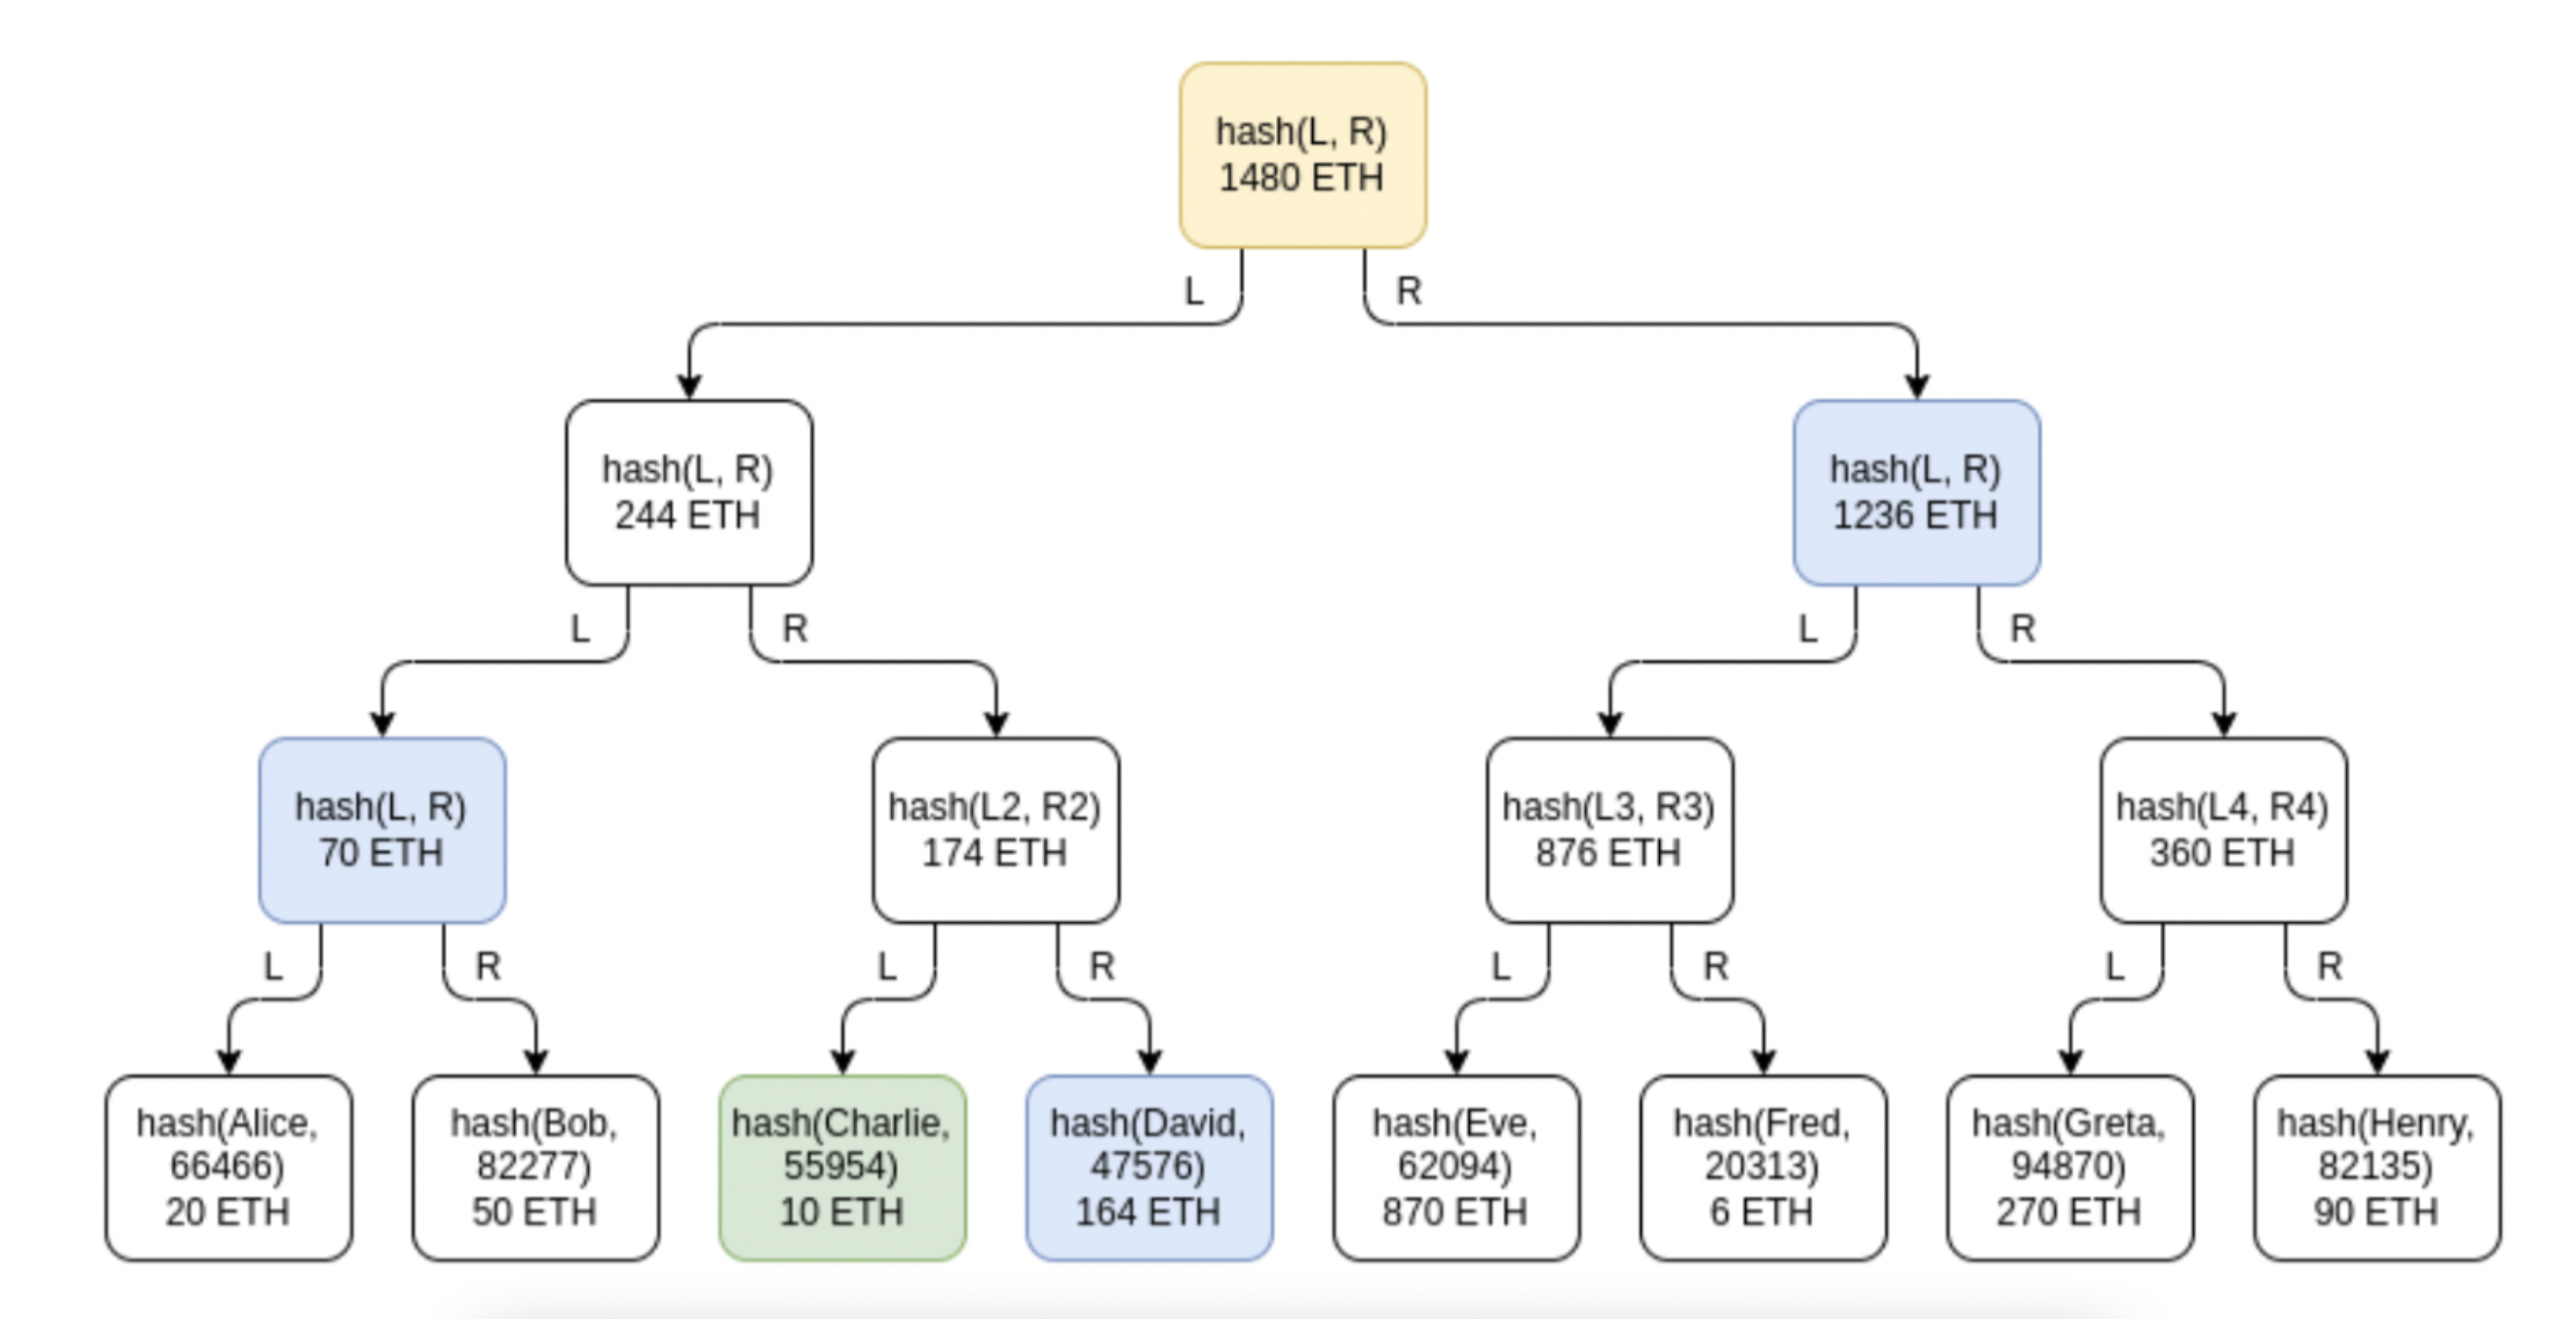
\includegraphics[width=70mm]{MerklePath.png}}
   \hfill
   \subfloat[Post change]{\includegraphics[width=70mm]{MerklePathTemp.png}}
   \hfill
   \caption{Merkle tree change}
   \end{figure}

For every change in the Merkle tree, we have the Merkle path with the old values, the new values, the temporary root hash, and the temporary root sum.
The \hyperref[subsec:plcc]{circuit} is iterating over the changes and gives a final root hash and final root sum. 
The circuit verifies each old path, updates the leaf with new values, recomputes the hash, and sums up the tree. 
The constraints enforce hash and sum calculations, valid path directions, and range checks.

The change circuit also follows the zero-knowledge \hyperref[subsec:zkp]{properties}. 
\paragraph{Properties}
\begin{itemize}
   \item Completeness: If the changes are valid, with correct old and new Merkle paths, an honest prover can generate a proof that convinces an honest verifier of the statement. Constraints on the paths and updates enforce this.
   \item Soundness: If any change is invalid or the old state is manipulated, no dishonest prover can produce valid proof because of the constraints.
   \item Zero-Knowledge: The verifier learns only the public outputs and nothing about the private inputs.
   \end{itemize}

\subsubsection{Minimizing the number of changes}
To minimize the number of constraints, we want to minimize the number of changes.
We define a change as a hash change at the leaf level. Any new user, balance change, or removal of the old user is considered a change.
The naive change calculation would be $changes = balanceChanges + newUsers + deprecateUser$.
However, a new user can take the node of a deprecated user. So we would have the equation $changes = balanceChanges + max(newUsers, deprecateUser)$. 
Constraints enforce this calculation, reducing the circuit's complexity by limiting updates.

\subsubsection{Constraint analysis}
The new circuit makes sense theoretically. It should be faster than the original one, so let us analyze it.
We want to compare the number of constraints in the original circuit with those in the changed circuit.
The first assumption is to assume the number of changes in a day. A completely arbitrary value would be $1\%$.
\begin{figure}[H]
   \centering
   \includegraphics[width=130mm]{Number of constraints.png}
   \caption{Number of constraints original circuit vs new circuit with 1\% change}
   \label{overflow}
   \end{figure}
Once you reach more than 128 users with $1\%$ change, it is not worth it to use the new circuit.
This is not practical because any marketplace will have more than 128 users.
However, we can see that the number of constraints of the new circuit grows linearly with the number of changes.
This means that two circuits with $0.5\%$ changes would have a similar number of constraints as one circuit with $1\%$ changes.
We can take this a step further and look at daily proof instead of hourly proof.
With the assumption that $1\%$ changes daily, we will assume that $0.05\%$ of the balances change hourly.
Let us look at the number of constraints if $0.05\%$ of users change every hour.
\begin{figure}[H]
   \centering
   \includegraphics[width=130mm]{Number of constraints .05.png}
   \caption{Number of constraints (millions) original circuit vs new circuit with 0.05\% change}
   \label{overflow}
   \end{figure}
Even with more than 1 million users, our new circuit has three times fewer constraints.
So, if we want to do an hourly proof, the new circuit is less expensive than the old circuit.
We can take this further and provide proof at every new block. We could have a Merkle tree up to date for the liabilities side at every block.

While the new circuit improves the hourly and block proofs, a daily proof may be sufficient for most use cases.
It is still less work to do the daily proof with the original circuit than 24 hourly proofs with the new circuit. 

\section{Daily proof of inclusion}
Because a marketplace can have millions of users, it is impractical to build a proof of inclusion for every user daily.
The user is responsible for requesting proof that their balance is included in the published Merkle tree.

Ideally, a Merkle tree would be published at least daily. However, it is once again impractical to require every user to verify their inclusion daily.
Nevertheless, each user verifying their inclusion in the tree increases the chance that the proof of liabilities is valid and includes every balance.
This is why it is primordial to find a way to make it easier to verify the inclusion. This is where Nova folding schemes come in.
Nova suggested using the folding scheme to verify the proof of inclusion from multiple rounds simultaneously\cite{NS23}. 
This is used in a zero-knowledge proof of reserves tool called Summa \cite{Summa24}.
They implemented a similar proof of inclusion to what we are working on. They have similar Merkle tree inputs, outputs and constraints. However, they 
use Halo2, and their circuit can handle multiple cryptocurrencies. Halo2 is an established tool for generating SNARKS, using Plonk instead of Groth16, like us.


The novel way to generate proof of inclusion is to generate a proof of inclusion that is valid from the day the account is created to the day the user requests it.
Normally, you would need to create 500 different proofs for 500 days. However, as we saw in the previous section, the Nova folding scheme enables combining 500 proofs into just one.
The folding scheme circuit compresses multiple proofs by combining their constraints.
Verifying this one proof is the equivalent of verifying the 500 or any other number of days required.
This drastically simplifies the verification process.

Previously, when requesting a proof of inclusion, the user would only receive proof that their balance is included in the latest published Merkle tree. Now, the proof verifies that the balance has been included in every previously published Merkle tree. 
This ensures that any malicious entity would be unable to alter ownership of balances across multiple days. 

It might seem like a small detail, but it is the detail that makes all the difference. Let us evaluate why.
In the initial round, with no changes, the failure probability for 20k users remains at $13\%$.

\begin{figure}[H]
   \centering
   \includegraphics[width=130mm]{FailureProbabilityRound1.png}
   \caption{Failure Probability Round 1 \cite{NS23}}
   \label{overflow}
   \end{figure}

However, if we have 20k distinct users in round 2, the failure probability of round 1 decreases to $1.6\%$.

\begin{figure}[H]
   \centering
   \includegraphics[width=130mm]{FailureProbabilityRound2.png}
   \caption{Failure Probability Round 1 After 2 Rounds \cite{NS23}}
   \label{overflow}
   \end{figure}

If we have 20k different users in round 3, the failure probability of round 1 further decreases to $0.2\%$.

\begin{figure}[H]
   \centering
   \includegraphics[width=130mm]{FailureProbabilityRound3.png}
   \caption{Failure Probability Round 1 after 3 Rounds \cite{NS23}}
   \label{overflow}
   \end{figure}
The key takeaway is that we require $4\%$ of users to verify every round without folding. However, with folding, we only need
$4\%$ of users to participate in at least 1 round. This significantly reduces the burden on the user to verify while increasing confidence in the proof.

\subsection{Circuit Design}
In order to implement folding, we need to adjust our \hyperref[subsec:pi]{circuit} slightly. Everything except the way we handle inputs and outputs stays the same.
The private inputs vary for every instance, while the public inputs are carried over from round to round. 
The circuit verifies the Merkle path for a user's balance, recomputing the root hash and sum via hashing.

\paragraph{Inputs}
\begin{itemize}
   \item List of neighbors sum (private): Sums of nearby Merkle tree nodes, kept secret to hide the tree structure.
   \item List of neighbors hash (private): Hashed values of nearby nodes, hidden to protect tree privacy.
   \item List of neighbors binary (private): Left/right indicators (0 or 1) for the Merkle path, kept secret to conceal path details.
   \item Root hash (private): Merkle tree's top value, hidden to maintain proof privacy.
   \item Root sum (private): Total balance sum, kept secret to protect aggregate data.
   \item User balance (private): User's balance, hidden to preserve individual privacy.
   \item User email hash (private): Hashed user email, kept secret to protect identity.
   \item Steps in (public): Public values from the previous circuit's output, shared to link folded rounds.
   \end{itemize}

\paragraph{Outputs}
\begin{itemize}
   \item Steps out (public): Public values passed to the next circuit, enabling folding across rounds.
   \end{itemize}

\paragraph{Steps}
\begin{itemize}
   \item Balance included: Confirms the user's balance is in the Merkle tree.
   \item Root sum: Total balance sum for the tree.
   \item Root hash: Merkle tree's top value.
   \item User balance: User's balance value.
   \item User email hash: Hashed user email.
   \end{itemize}

All the data passed around between the circuits is public and is called step in and step out, while the regular inputs are private.
The step in of a circuit is the step out of the previous one.

\begin{figure}[H]
   \centering
   \includegraphics[width=130mm]{FoldingCircuit.png}
   \caption{Folding Circuit}
   \label{overflow}
   \end{figure}

S0 is the step in of the first change, S1 is the step out of the first change and the step in of the second change. $F$ is the folded circuit
and $T$ is the number of times it is folded.

These steps encompass all the public values we initially had in the circuit.
None of the variables of the steps are used in the circuit itself. They are used to make a value public.

The initial circuit takes meaningless values as inputs, while the following circuits take the public values of the previous circuit.
In the end, we only have to verify a single proof. We must also compare the circuit output with the proof of liabilities outputs for every round.

\section{Folded daily proof of liabilities}
With the original circuit, we saw that folding or any other recursion scheme was ineffective.
However, with the new circuit, we were able to separate a big proof into multiple smaller ones.
This aligns perfectly with the recursion ideas.
We can separate our new circuit of $n$ changes into $m$ circuits, where $m <= n$, and fold the circuits together. 
The folding process combines constraints from each circuit.

\begin{figure}[H]
   \centering
   \includegraphics[width=130mm]{Proof time.png}
   \caption{Proof time original circuit vs folded circuit with 1\% change, 1 change by fold}
   \label{overflow}
   \end{figure}

After 10,000 users, both circuits grow linearly, with the folded circuit doing much better. For instance,
for 1M users, the old circuit takes 196,608 seconds, and the new circuits take 17 188 seconds. This is more than 10 times better.
We should take the number of seconds with a grain of salt since these measurements were done on my Mac, and there are much more performant computers.
The data we should focus on is that the folded circuit took 10x less time, and it was not even optimized. We were doing one change by circuit, so at 1M users, we folded 10k circuits.

Now that we know our circuit is better, we can optimize it.

\begin{figure}[H]
   \centering
   \includegraphics[width=130mm]{Proof time vs verifier time.png}
   \caption{Optimization of the proof time and verifier time of the folded circuit with 1\% change and 1M users}
   \label{overflow}
   \end{figure}

As we can see, the optimal time for the prover is between 8 and 32 changes by fold, while the verifier time seems to be growing at a monotonic pace.
We can decide the number of changes we should have for every fold depending on the use case.

\subsection{Circuit design}
The folded change circuit is the same as the regular change circuit, but the inputs work differently because some data is passed around the circuits.
There are two types of step variables: those needed in the following circuit and those just there to be public.
Starting from the inputs of the regular change circuit, the old hash and old sum root are moved to the step in, while all the outputs are moved to step out. 
The circuit processes each change by verifying old paths, updating leaves, and recomputing hashes and sums.

\paragraph{Inputs}
\begin{itemize}
   \item List of old email hash (private) - 1 per change: Hashed user email from the previous tree, kept secret to protect identities.
   \item List of old values (private) - 1 per change: Previous balances, hidden to preserve privacy.
   \item List of new email hash (private) - 1 per change: Updated hashed email, kept secret for user confidentiality.
   \item List of new values (private) - 1 per change: Updated balances, hidden to protect amounts.
   \item List of temporary root hash (private) - 1 per change: Intermediate tree top values, kept secret to hide updates.
   \item List of temporary root sum (private) - 1 per change: Intermediate balance sums, hidden for privacy.
   \item List of neighbors sum (private) - 1 list per change: Sums of nearby nodes in Merkle paths, kept secret to conceal tree structure.
   \item List of neighbors hash (private) - 1 list per change: Hashed nearby nodes in Merkle paths, hidden for privacy.
   \item List of neighbors binary (private) - 1 list per change: Left/right indicators (0 or 1) for Merkle paths, kept secret to protect path details.
   \item Step in (public): Public values from the previous circuit, shared to link folded circuits.
   \end{itemize}

\paragraph{Outputs}
\begin{itemize}
   \item Steps out: Public values passed to the next circuit, enabling folding.
   \end{itemize}

\paragraph{Steps}
\begin{itemize}
   \item Valid hash and valid sum: Confirms the new hash and sum are correct.
   \item All small range: Ensures balances are non-negative and within safe limits.
   \item Root hash: Final Merkle tree top value.
   \item Root sum: Final total balance sum.
   \end{itemize}




%Mina proof of recursion
%summa
%https://summa.gitbook.io/summa/v/1/circuits/Merkle-sum-tree-inclusion
%https://www.youtube.com/watch?v=sRAA1RYYHEs
%https://hackmd.io/@summa/HkGMF4Ovn#The-problem
